\documentclass{article}
\usepackage{amsmath}
\usepackage{float}
\usepackage{fvextra} 
\usepackage{datetime}
\usepackage{graphicx}


\title{Mechine Learning - Assignment 3}
\author{Michael Dadush \\ 206917908 \and Shay Gali \\ 315202242}
\date{\monthname[\month] \ \the\year}

\begin{document}
\maketitle

\section{K-Nearest Neighbors Classifier}

Based on our experiment results with different k-nearest neighbor parameters, we can make important observations about the classifier performance. We will analyze the results for different k and p values.


\subsection{Code Output}
This is the code output for different k and p values:
\begin{Verbatim}[fontsize=\small, xleftmargin=0pt, xrightmargin=0pt]
    round       | Average Empirical Errors  |  Average True Errors  |  Error Differences
p = 1   k = 1   |         0.014600          |       0.130800        |      0.116200
p = 1   k = 3   |         0.055800          |       0.093800        |      0.038000
p = 1   k = 5   |         0.060400          |       0.090000        |      0.029600
p = 1   k = 7   |         0.063800          |       0.090000        |      0.026200
p = 1   k = 9   |         0.065400          |       0.090000        |      0.024600
                |                           |                       |
p = 2   k = 1   |         0.014800          |       0.126200        |      0.111400
p = 2   k = 3   |         0.054400          |       0.092000        |      0.037600
p = 2   k = 5   |         0.062800          |       0.085400        |      0.022600
p = 2   k = 7   |         0.064200          |       0.085200        |      0.021000
p = 2   k = 9   |         0.063600          |       0.084400        |      0.020800
                |                           |                       |
p = inf k = 1   |         0.014800          |       0.136200        |      0.121400
p = inf k = 3   |         0.056600          |       0.090400        |      0.033800
p = inf k = 5   |         0.062400          |       0.085200        |      0.022800
p = inf k = 7   |         0.063000          |       0.086400        |      0.023400
p = inf k = 9   |         0.065400          |       0.084200        |      0.018800
\end{Verbatim}


\subsection{Best Parameters}
From looking at the data results, we found that the best parameters are:
\begin{itemize}
    \item p = 2 with k = 9 (error rate = 0.0844 or 8.44\%)
    \item Also good is p = $\infty$ with k = 9 (error rate = 0.0842 or 8.42\%)
\end{itemize}

These parameters give us the lowest Average True Errors, which is most important for real performance.

\subsection{Analysis of k Parameter}
When we look at how k affects the results:
\begin{itemize}
    \item k = 1 gives worst performance on test data for all p values
    \item When k gets bigger, the true error usually gets smaller
    \item This shows us that using more neighbors helps make better predictions
\end{itemize}

\subsection{Analysis of p Parameter}
For the distance metric p:
\begin{itemize}
    \item p = 1 does not work as good as p = 2 or p = $\infty$
    \item p = 2 (Euclidean) and p = $\infty$ work almost same, but p = 2 is little better
    \item We think this shows that using regular distance (p = 2) works better for our data than other options
\end{itemize}

\subsection{Overfitting Analysis}
We see clear overfitting in our results, especially with k = 1:

For k = 1:
\begin{itemize}
    \item Very small empirical errors ($\approx$ 0.014-0.015)
    \item Much bigger true errors ($\approx$ 0.126-0.136)
    \item Big differences between errors ($\approx$ 0.111-0.121)
\end{itemize}

When k gets bigger:
\begin{itemize}
    \item Empirical errors get little bigger
    \item True errors get much smaller
    \item Differences between errors get smaller too
\end{itemize}

This pattern shows classic overfitting when k = 1. The model learns training data too well (small empirical error) but cannot work good on new data (big true error). Using bigger k helps fix this by taking average of more neighbors.

\subsection{Why These Parameters Work Best}
k = 9 with p = 2 gives best results because:
\begin{itemize}
    \item It uses enough neighbors to make predictions more stable
    \item It reduces overfitting (smallest difference between empirical and true errors)
    \item Euclidean distance (p = 2) seems to work better for relationships between features than Manhattan (p = 1) or maximum distance (p = $\infty$).
    \item Euclidean distance represents how the human eye sees distances, which is good for our data
    \item The big k value (k = 9) tells us there is probably lot of noise in data that needs to be averaged
\end{itemize}

\subsection{Conclusion}
Our analysis shows that k = 9 and p = 2 give best performance for this classification task. These parameters help balance between learning from data and not overfitting. The results also show importance of choosing right k value to avoid overfitting, especially avoiding k = 1 which memorizes training data too much.

\section{Decision Tree Classifier}

We tested two ways to build decision trees: brute-force and binary entropy. Both methods were limited to 3 levels (k=3). We used the Iris dataset and focused on separating Iris-versicolor (marked as 0) from Iris-virginica (marked as 1).

\subsection{Results}

Our accuracy results were:
\begin{itemize}
    \item Brute force method: 95\%
    \item Binary entropy method: 93\%
\end{itemize}

\subsection{The Trees We Got}

You can see both trees in Figures \ref{fig:brute_force_tree} and \ref{fig:entropy_tree}.

\begin{figure}[H]
    \centering
    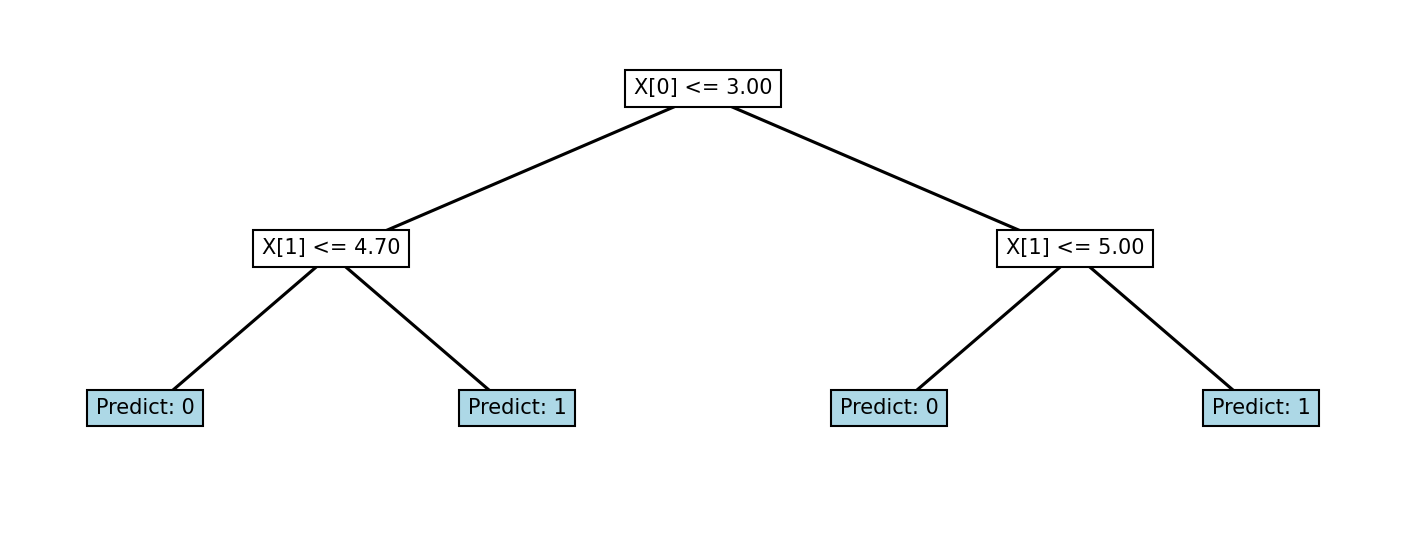
\includegraphics[width=0.8\textwidth]{assets/brute_force_tree.png}
    \caption{The tree from brute force method}
    \label{fig:brute_force_tree}
\end{figure}

\begin{figure}[H]
    \centering
    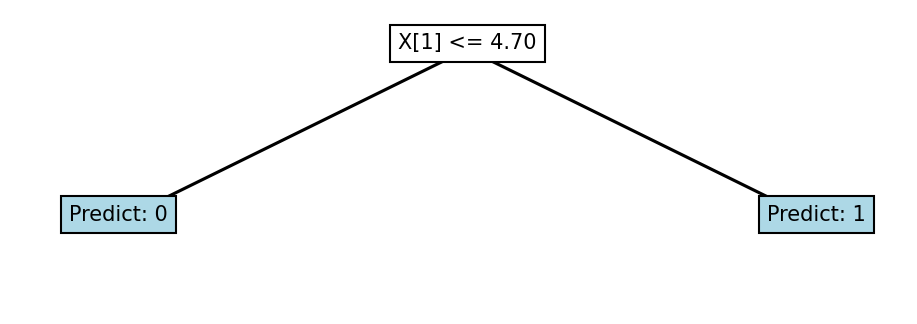
\includegraphics[width=0.8\textwidth]{assets/entropy_tree.png}
    \caption{The tree from entropy method}
    \label{fig:entropy_tree}
\end{figure}

\subsubsection{Analyze the results}

Let's look at what each method did:

\paragraph{Brute Force Method}
\begin{itemize}
    \item Got better accuracy (95\%)
    \item Used all 3 levels we allowed - need both features to make the decision (the VC dimension is 2)
    \item Made these splits:
        \begin{itemize}
            \item First split: X[0] $\leq$ 3.00
            \item Left side: X[1] $\leq$ 4.70
            \item Right side: X[1] $\leq$ 5.00
        \end{itemize}
\end{itemize}

\paragraph{Binary Entropy Method}
\begin{itemize}
    \item Got 93\% accuracy
    \item Used just two level even though it could use three - we need only one feature to make the decision
    \item Made one split: X[1] $\leq$ 4.70
\end{itemize}

\paragraph{Comparing the Methods}
The entropy method made a much simpler tree and still worked almost as well (only 2\% worse). This tells us:
\begin{itemize}
    \item The simpler tree might work better on new data
    \item X[1] is probably the more important feature
    \item The brute force tree might be too complex for what we need
\end{itemize}

\noindent For real use, we think the entropy method is better because it's simpler and faster, even though it got slightly lower accuracy. The brute force method might be trying too hard to fit our specific data.
\end{document}